\documentclass[11pt]{article}

\usepackage[a4paper,margin=27mm]{geometry}
\usepackage{amsmath,amssymb,amsthm,mathtools}
\usepackage{array}
\usepackage{booktabs}
\usepackage{longtable}
\usepackage{graphicx}
\usepackage{xcolor}
\usepackage{xr-hyper}
\usepackage[hidelinks]{hyperref}
\usepackage{microtype}
\usepackage[T1]{fontenc}
\usepackage{lmodern}
\setlength{\emergencystretch}{2em}

\externaldocument[main-]{manuscript}
\newcommand{\norm}[1]{\left\lVert #1\right\rVert}
\newcommand{\C}{\mathbb{C}}
\newcommand{\R}{\mathbb{R}}
\newtheorem{theorem}{Theorem}
\newtheorem{corollary}[theorem]{Corollary}
\newtheorem{proposition}[theorem]{Proposition}

\renewcommand{\thesection}{S\arabic{section}}
\renewcommand{\thesubsection}{\thesection.\arabic{subsection}}
\renewcommand{\thefigure}{S\arabic{figure}}
\renewcommand{\thetable}{S\arabic{table}}
\renewcommand{\theequation}{S\arabic{equation}}

\begin{document}

\title{Supplemental Material for\\
Band Equivalence Does Not Determine Hopping Locality:\\
Exact Rank-Two Geometry and Equal-Accuracy Range Inflation}
\author{Eugene Joseph M. Ragasa\\
Department of Physics, De La Salle University, Manila, Philippines\\
\texttt{eugene.ragasa@dlsu.edu.ph}}
\date{Working Physical Review B revision --- 16 October 2026}
\maketitle

\noindent This supplement contains analytic derivations, the formal alignment contract,
numerical-resolution and verification details, diagnostic figures, a separately retained
scalar Fourier-reduction precursor, the claim--evidence register, and execution procedures
supporting the main manuscript. Prospective controls
and development results retain the scientific status stated in the main text.

\tableofcontents
\clearpage
\section{Analytic proofs}
\subsection{Exact loss geometry}
\begin{proof}[Proof of Theorem~\ref{main-thm:exact-loss-geometry}]
Let $d_{ia}=h_a(q_i)-\bar E(q_i)$. Since $D(q_i)$ is traceless,
$d_{i1}+d_{i2}=0$. Equation~\eqref{main-eq:candidate-eigenvalues} gives the normalized
spectral residual
\[
 s+(\lambda-1)d_{ia}/E_{\mathrm{ref}}.
\]
When its square is summed over the two retained states, the term linear in $s(\lambda-1)$
vanishes because the two $d_{ia}$ sum to zero. The remaining splitting term is
\[
 \sum_i\frac{\alpha_i}{2E_{\mathrm{ref}}^2}\sum_a d_{ia}^2
 =\sum_i\frac{\alpha_i}{2E_{\mathrm{ref}}^2}\norm{D(q_i)}_F^2
 =\kappa,
\]
which proves Eq.~\eqref{main-eq:exact-spectral-loss}.

For the operator channel, Eqs.~\eqref{main-eq:attacked-matrix} and
\eqref{main-eq:global-alignment} give the normalized matrix residual
\[
 sI_2+\frac{\lambda D_{i,\phi}-B_i}{E_{\mathrm{ref}}}.
\]
The cross term containing $s$ vanishes because both $D_{i,\phi}$ and $B_i$ are
traceless. Unitary invariance of the Frobenius norm gives
$\norm{D_{i,\phi}}_F=\norm{B_i}_F=\norm{D(q_i)}_F$. Expansion therefore yields
\[
 L_{\mathrm{op},\phi}^2
 =s^2+\kappa\lambda^2-2b_\phi\lambda+\kappa.
\]
Completing the square and using $\mu_\phi=b_\phi/\kappa$ proves
Eq.~\eqref{main-eq:exact-operator-loss}. Finally, Cauchy--Schwarz in the weighted Frobenius
inner product gives $|b_\phi|\le\kappa$, hence $|\mu_\phi|\le1$.
\end{proof}

\subsection{Compatibility and exact ellipse distance}
\begin{proof}[Proof of Corollary~\ref{main-cor:compatibility-distance}]
Use the scaled coordinates $x=s$ and $y=\sqrt{\kappa}\lambda$. By
Theorem~\ref{main-thm:exact-loss-geometry}, the spectral ellipse becomes a disk of radius
$\tau_s$ centered at $(0,\sqrt{\kappa})$. The continuously optimized operator ellipse
becomes a disk of radius $r_*$ centered at
$(0,\sqrt{\kappa}\mu_{\max})$. Two disks intersect exactly when the distance between
their centers does not exceed the sum of their radii, which is
Eq.~\eqref{main-eq:exact-intersection}. Their centers differ only along the splitting
coordinate, so transforming the positive disk gap back to $(s,\lambda)$ coordinates
gives Eq.~\eqref{main-eq:exact-distance}.
\end{proof}

\subsection{Constructed band-only false positive}
\begin{proof}[Proof of Proposition~\ref{main-prop:constructed-fail}]
For this construction, $\kappa=1$. Conjugation of $\sigma_z$ by a real rotation changes
its orientation through twice the rotation angle. Equation~\eqref{main-eq:operator-correlation}
therefore gives
\[
 \mu_\phi
 =\frac12\left[\cos(2\phi)+\cos\left(\frac\pi2-2\phi\right)\right]
 =\frac{1}{\sqrt2}\cos\left(2\phi-\frac\pi4\right).
\]
Hence the largest attainable positive correlation is
$\mu_{\max}=1/\sqrt2$, reached at $\phi=\pi/8$. The spectral admissible ellipse is
\[
 s^2+(\lambda-1)^2\le0.05^2.
\]
At the best global angle, the operator ellipse is
\[
 s^2+\left(\lambda-\frac1{\sqrt2}\right)^2
 \le 0.72^2-\frac12.
\]
Both ellipses lie inside $X$. Their centers differ only along the splitting coordinate,
so Corollary~\ref{main-cor:compatibility-distance} gives
Eq.~\eqref{main-eq:constructed-fail-distance}.

Angles with smaller positive $\mu_\phi$ cannot reduce the separation: wherever their
operator component is nonempty, decreasing $\mu_\phi$ moves its center farther from
$\lambda=1$ and does not compensate for that shift through its radius. Components with
negative $\mu_\phi$ are either empty at the stated threshold or lie entirely below
$\lambda=0.50$. Thus no allowed global angle produces a joint witness in $X$.
\end{proof}

\subsection{Smooth threshold continuum}
\begin{proof}[Proof of Corollary~\ref{main-cor:threshold-continuum}]
For $D=E_{\mathrm{ref}}\sigma_z$, conjugation through Eq.~\eqref{main-eq:attack-continuum} gives
\[
 U_a(q)^\dagger D U_a(q)
 =E_{\mathrm{ref}}\left[
  \cos\!\left(2a\sin2\pi q\right)\sigma_z
  -\sin\!\left(2a\sin2\pi q\right)\sigma_x
 \right].
\]
The sine term has zero reciprocal-period average, while the cosine average is
$J_0(2a)$. A global rotation aligned with $\sigma_z$ therefore maximizes the operator
correlation and proves Eq.~\eqref{main-eq:continuum-correlation}. Substitution into
Theorem~\ref{main-thm:exact-loss-geometry} gives
Eq.~\eqref{main-eq:minimum-operator-threshold}. Solving the exact disk-intersection condition
in Eq.~\eqref{main-eq:exact-intersection} gives
Eqs.~\eqref{main-eq:joint-threshold-continuum} and
\eqref{main-eq:exact-spectrum-threshold-continuum}. On the stated interval, $2a$ remains
before the first positive zero of $J_0$, and $J_0(2a)$ decreases monotonically; the
thresholds therefore increase monotonically.
\end{proof}

\subsection{Residual--locality identity}
\begin{proof}[Proof of Theorem~\ref{main-thm:residual-locality-identity}]
Every matrix $U(q)^\dagger D U(q)$ is traceless, has Frobenius norm $\norm D_F$, and lies
in the two-dimensional real rotation orbit of $D$. Its average $B_0$ lies in the disk
spanned by that orbit. Hence there are a global angle $\phi_0$ and a scale
$\lambda_0\ge0$ such that
\[
 B_0=\lambda_0R(\phi_0)^\dagger D R(\phi_0),
 \qquad
 \lambda_0=\frac{\norm{B_0}_F}{\norm{D}_F}=\mu_{\max}.
\]
The best constant globally aligned field is therefore the orthogonal projection $B_0$.
The trace shift is minimized by $s=0$, and
\begin{equation}
 \inf_{s,\lambda,\phi}L_{\mathrm{op},\phi}^2
 =\frac{1}{2E_{\mathrm{ref}}^2}
  \int_{-1/2}^{1/2}\norm{B(q)-B_0}_F^2\,dq.
 \label{eq:mean-field-residual}
\end{equation}
Parseval's identity applied entrywise to
Eq.~\eqref{main-eq:continuous-traceless-fourier} turns the right side into the nonzero-mode
sum in Eq.~\eqref{main-eq:residual-locality-right}. Unitary invariance gives
$\norm{B(q)}_F=\norm{D}_F$ pointwise, so a second application of Parseval gives
\[
 \sum_{R\ne0}\norm{B_R}_F^2
 =\norm D_F^2-\norm{B_0}_F^2
 =\norm D_F^2(1-\mu_{\max}^2).
\]
Division by $2E_{\mathrm{ref}}^2$ proves Eq.~\eqref{main-eq:residual-locality-left}.
\end{proof}

\subsection{Admissible-alignment covariance and its distinction from MLWF spread}
\label{sec:alignment-covariance}

This subsection records a comparison-contract property used to interpret the restricted
operator loss. It is included for self-containment, not as a new localization theorem.
Let $V_{\mathrm{ref}}$ and $V_{\mathrm{red}}$ be finite-dimensional retained spaces of
equal rank, let $\mathcal S$ be a finite translation inventory, let $\omega_R>0$, and
fix $Z_{\mathrm{ref}}>0$. For a nonempty declared family $\mathcal U$ of unitary
identification maps $C:V_{\mathrm{red}}\to V_{\mathrm{ref}}$, define
\begin{equation}
 \mathcal L_H(C,\vartheta)
 =\frac{1}{Z_{\mathrm{ref}}}
  \sum_{R\in\mathcal S}\omega_R
  \norm{H_{\mathrm{ref}}(R)
  -C H_{\mathrm{red}}(R;\vartheta)C^\dagger}_F^2.
 \label{eq:generic-alignment-loss}
\end{equation}
The inventory, weights, normalization, represented state spaces, and admissible family
are all part of the frozen comparison contract.

\begin{proposition}[Attainment, transported-frame covariance, and excess]
\label{prop:alignment-covariance}
If $\mathcal U$ is compact, the continuous finite loss in
Eq.~\eqref{eq:generic-alignment-loss} attains a minimum. Define
\begin{align}
 \mathcal L_{H,\min}(\vartheta)
 &=\min_{C\in\mathcal U}\mathcal L_H(C,\vartheta),\\
 \mathcal L_{H,\mathrm{excess}}(C_0,\vartheta)
 &=\mathcal L_H(C_0,\vartheta)-\mathcal L_{H,\min}(\vartheta),
 \qquad C_0\in\mathcal U.
\end{align}
Then $\mathcal L_{H,\mathrm{excess}}\ge0$. Under independent constant unitary frame
changes $A$ on $V_{\mathrm{ref}}$ and $B$ on $V_{\mathrm{red}}$, transport both the
operators and the admissible family according to
\begin{align}
 H_{\mathrm{ref}}'(R)&=AH_{\mathrm{ref}}(R)A^\dagger,\\
 H_{\mathrm{red}}'(R;\vartheta)&=BH_{\mathrm{red}}(R;\vartheta)B^\dagger,\\
 \mathcal U'&=\{ACB^\dagger:C\in\mathcal U\}.
\end{align}
The minimum loss is unchanged, and corresponding selected maps
$C_0'=AC_0B^\dagger$ have the same excess.
\end{proposition}

\begin{proof}
Continuity on compact $\mathcal U$ gives attainment by the extreme-value theorem, and
nonnegativity of the excess follows from the defining minimum. For
$C'=ACB^\dagger$, the transformed residual is
\begin{equation}
 H_{\mathrm{ref}}'(R)-C'H_{\mathrm{red}}'(R;\vartheta)C'^\dagger
 =A\left[H_{\mathrm{ref}}(R)
 -CH_{\mathrm{red}}(R;\vartheta)C^\dagger\right]A^\dagger.
\end{equation}
Unitary invariance of the Frobenius norm gives
$\mathcal L_H'(C',\vartheta)=\mathcal L_H(C,\vartheta)$. The map
$C\mapsto ACB^\dagger$ is a bijection from $\mathcal U$ to $\mathcal U'$, so taking the
minimum proves covariance of the minimum. Subtracting equal minima from the losses of
corresponding selected maps proves covariance of the excess.
\end{proof}

The proposition does \emph{not} reproduce or strengthen the MLWF spread decomposition
$\Omega=\Omega_{\mathrm I}+\widetilde\Omega$~\cite{marzari1997,marzari2012}. In that
established construction, $\Omega_{\mathrm I}$ is determined by the retained subspace
projectors and $\widetilde\Omega$ depends on the selected Bloch frame; the variational
problem concerns spatial spread and Wannier localization. By contrast,
Eq.~\eqref{eq:generic-alignment-loss} compares two represented Hamiltonians over a
contract-specific set of identification maps. Its minimum is not an intrinsic
projector functional, and its excess is merely the nonnegative scalar difference from
the declared minimum, not an orthogonal decomposition of either an operator residual or
a Wannier spread. Transported-frame covariance does not authorize enlargement of
$\mathcal U$, identify a physically preferred gauge, or admit momentum-dependent
alignments excluded by the contract. If the retained ranks differ or $\mathcal U$ is
empty, this matrix-subtraction channel instead requires an explicitly authorized
embedding or is undefined.

For the active benchmark, $\mathcal U$ is the compact one-parameter family of global
real rotations modulo its period. The main analytic results do more than invoke
Proposition~\ref{prop:alignment-covariance}: they evaluate that restricted minimum
exactly and relate it to induced non-onsite Fourier weight.

\section{Numerical resolution and convergence}

\subsection{Nested construction meshes}

The draft construction-mesh ladder is
\begin{equation}
 N\in\{32,64,128,256,512\},
 \qquad
 q_i=-\frac12+\frac{i}{N},
 \quad i=0,\ldots,N-1.
 \label{eq:construction-meshes}
\end{equation}
Here $N$ is the number of momentum samples in one reciprocal-space quadrature, not the
number of independent model calculations. For example, $N=64$ means that the single
matrix-valued function $K(q)$ is assembled and diagonalized at 64 distinct momenta. The
matrices differ because the phase $e^{2\pi iqR}$ differs at each momentum. No parent
parameter is refitted between points.

The momentum grids are nested under doubling: every point on an $N$-point grid is an
even-index point on the $2N$-point grid. Reuse of previous evaluations means that a
complete refinement through $N=512$ contains 512 unique construction momenta rather than
the sum of all mesh sizes.

The completed flat-parent convergence study uses one fixed set of 65 amplitudes at every
momentum resolution. Its `converged' disposition concerns momentum refinement only. It
compares finite-mesh maximum correlation, the two thresholds, non-onsite hopping weight,
shared-block Fourier power, maximizing-angle status, the finite-mesh--Bessel quadrature
discrepancy, band discrepancy, the three-way identity discrepancy, and Parseval discrepancy. The discrete
$\mu_{N,\max}(a)$ and analytic $J_0(2a)$ remain separate. The analytic continuum shown
in Fig.~\ref{fig:flat-parent-analysis}(a,b) is evaluated directly and is not an
amplitude-interpolation disposition.

The non-flat convergence implementation compares the sampled external isolation gap,
shared-node parent eigenvalues and retained spectral projectors, frame orthonormality and
closure, Hermiticity, harmonic maximum and maximizing-angle status, $\mu_{N,\max}$, the
two thresholds, Fourier-block powers, non-onsite weight, band discrepancy, quadratic
reconstruction, and Parseval consistency. The neighboring-frame transport singular
value is a per-mesh rank-qualification lower bound, not a convergence observable. The
study has no $J_0(2a)$ analytic comparator and does not assume the flat-parent three-way
locality identity. Full parent eigenvalue and projector arrays, admissible-set
quadratics, rectangle minima, witness coordinates,
support points, containment margins, separation bounds, and post-decision evaluation
losses remain unimplemented. Current non-flat conclusions are pointwise at directly
evaluated amplitudes. Any future continuous-amplitude claim must invoke a reviewed
adaptive rule with explicit thresholds and caps.

For a scalar, vector, or matrix quantity $z$, the draft continuous convergence test is
\begin{equation}
 \norm{z_{\mathrm{fine}}-z_{\mathrm{coarse}}}_\infty
 \le
 \epsilon_{\mathrm{abs}}
 +\epsilon_{\mathrm{rel}}
  \max\!\left(1,\norm{z_{\mathrm{fine}}}_\infty\right),
 \label{eq:convergence-test}
\end{equation}
with draft values
$\epsilon_{\mathrm{abs}}=10^{-10}$ and
$\epsilon_{\mathrm{rel}}=10^{-8}$. These are deterministic numerical tolerances, not
physical error bars or probabilistic confidence limits.

For the completed flat-parent momentum study, every implemented continuous channel must
pass on two successive refinements and maximizing-angle status must remain unchanged on
the corresponding three levels. For a final non-flat study, every continuous
quantity must pass on two successive refinements, every discrete disposition must remain
unchanged on three successive levels, and every decisive threshold or separation margin
must be at least ten times larger than the corresponding observed refinement change. If
the applicable momentum or amplitude cap is reached first, qualification fails. The
largest attempted mesh is not called converged merely because no larger calculation was
performed.

\subsection{Disjoint post-decision evaluation}

After the construction size $N_*$ has been selected, the evaluation mesh has size
\begin{equation}
 M=4N_*+1
 \label{eq:evaluation-size}
\end{equation}
and coordinates
\begin{equation}
 \widetilde q_\ell=-\frac12+
 \frac{\ell+1/(N_*+1)}{M},
 \qquad \ell=0,\ldots,M-1.
 \label{eq:evaluation-mesh}
\end{equation}
The rational offset makes these coordinates distinct from the construction coordinates.
A future retained implementation must additionally check all coordinate separations in
the physical reciprocal unit against a fixed tolerance.

For the full non-flat workflow, the disposition, witness, alignment, and
separation certificate are fixed before the evaluation mesh is examined. Reference and
comparison matrices at evaluation coordinates are reconstructed from the finite Fourier
representation obtained on the construction mesh. The selected candidate is then
evaluated without refitting. This procedure probes interpolation and aliasing behavior
between construction nodes. It creates no statistical independence, estimates no
experimental uncertainty, and does not validate the parent model. The current smooth
implementations neither assign a post-decision admissible-set disposition nor execute
this workflow. The exploratory finite-range action does execute the disjoint mesh, but
issues neither an admissible-set disposition nor retained evidence.

\section{Independent verification and reproducibility}

\subsection{Numerical owners for this development snapshot}

The development implementation represented by this manuscript snapshot consumed the
exact revisions
\begin{center}
\small
\texttt{projectkoios-optimization}\\
\texttt{7ac5376bcb97e29f6927dda4d4ef714ed2e32140}\\[2pt]
\texttt{projectkoios-physkit}\\
\texttt{ed2e8118db9902316797d270305456735fab9712}.
\end{center}
Optimization owns continuous harmonic maximization and each complex-unitary pairwise
Procrustes solve in the producer. A numerically deficient overlap returns singular and
rank evidence but no full unitary transformation; KSD then applies the stricter declared
transport-overlap qualification gate. PhysKit owns immutable matrix-valued hopping
records, raw block Frobenius powers, and unit-aware complete bands from block-hopping
Bloch evaluations. PhysKit's band actions consume the canonical Numerics multi-series Fourier and batched
Hermitian-spectrum solvers and retain the correlated Bloch matrices, spectra, numerical
diagnostics, and backend evidence. The finite-range consequence action calls PhysKit's
ordered range-family evaluator so each source and its 17 cutoff models share one
reciprocal-grid phase matrix and one concatenated complete-spectrum solve. KSD supplies the finite-mesh identities, divides raw
powers by the retained rank and $E_{\mathrm{ref}}^2$, checks Parseval consistency, and interprets the
resulting locality and band-error channels.

PhysKit's hopping contracts use ordinary integer-lattice displacement semantics. The
complete even-$N$ Fourier inventory in this experiment remains cyclic and aliased: the
centered Nyquist representative $-N/2$ is self-conjugate only modulo $N$. KSD therefore
retains the cyclic Hermiticity check for the complete finite inventory. Any later
ordinary-lattice truncation must use a conjugate-closed retained set with
$R_c<N/2$, excluding the Nyquist representative. No owner API converts the finite
coefficients into continuous hoppings without a convergence argument.

\subsection{Independent numerical reconstruction}

The implemented flat-parent verifier reads canonical input and result records but does
not call the producing experiment action or trust a serialized disposition. It
independently reconstructs the sampled matrices, band discrepancy, second-harmonic
coefficients, continuous maximum and unique-or-degenerate angle status, finite-mesh and
analytic correlations, thresholds, Fourier-block powers, non-onsite weight, Parseval
identity, and flat-parent three-way identity. Its convergence verifier separately
reconstructs every adjacent momentum-mesh comparison and the final `converged' or
`unresolved' disposition.

The implemented `SmoothFourStateVerifier' independently reconstructs
Eq.~\eqref{main-eq:parent-bloch}, repeats the eigensystem and frame checks, reconstructs the
comparison field, Fourier blocks, Parseval quantities, and original restricted-alignment
loss, and obtains the harmonic maximum directly as
$b_0+\sqrt{c^2+d^2}$ without calling the producer's Optimization maximizer. A future
full verifier must additionally rebuild $Q$, $g$, and $c$ from
Eq.~\eqref{main-eq:quadratic}; recompute rectangle minima; check witness membership; derive
support points through linear solves; verify containment; reconstruct lower and upper
separation bounds; and apply
Eqs.~\eqref{main-eq:forward-fourier}--\eqref{main-eq:locality} to disjoint evaluation channels.
Those certificate checks lie outside the current four-state coverage.

The implemented `SmoothFourStateTruncationVerifier' independently reconstructs the
parent frames, finite Fourier blocks, centered-Nyquist conversion, ordinary-lattice
truncations, Bloch matrices, spectra, matrix and spectral error channels, and separate
first-passing cutoff decisions. It does not call the producing truncation action or
PhysKit's range-family evaluator. Its largest discrepancy on the dense development grid
is $4.61\times10^{-13}$.

Verification reports contain channel-resolved maximum discrepancies rather than only a Boolean
pass flag. Dimensionless discrepancies and energy-valued discrepancies remain separate. The main
calculation and verifier share binary64 arithmetic and may share numerical libraries;
that dependence is disclosed. Independence here means separate scientific
reconstruction and control flow, not independent hardware or an unrelated eigensolver.

\subsection{Serialization and calculation records}

The implemented flat-parent, non-flat, and truncation input, result, and verification
records use strict JSON schemas that reject unknown fields. The truncation records bind
conversion, interpolation, deliberate-truncation, total-error, and separate
range-decision channels; their scope fields expressly deny protocol freeze, provenance,
retained execution, and material validation. Retained schemas and the additional fields
needed by the future full admissible-set and separation-certificate workflow are deferred
until those contracts are reviewed. Numeric strings and Boolean values presented as real
numbers are rejected by the applicable public contracts.
Floating-point values must be finite. Complex values are represented by explicit real
and imaginary components, and arrays carry fixed dimensions wherever shape is part of
the scientific contract.

The active result records the SHA-256 digest of the exact canonical input bytes. The
verification record binds both input and result digests. Family, schema, and method
identities are checked against expected values rather than trusted from the payload, and
the input scope explicitly states that the calculation is not retained. Any change to a
nested value or immutable identity either changes the digest or fails schema validation.
A retained schema must additionally bind immutable version and run identities; the
development records carry no such inferred identity.

A retained run directory will be created by an exclusive no-overwrite operation. It will
contain canonical input, result, and verification records; the complete convergence table;
source and dependency provenance; platform and command information; authenticated
schema identities; the exact source manifest; a checksum manifest; and a readable
report separating controls, calculated quantities, and interpretation. Experiment
version, run identity, and content-addressed evidence-package identity remain distinct.

\subsection{Failure policy}

The active flat-parent calculation fails closed on nonfinite data, invalid dimensions,
malformed amplitudes or reciprocal meshes, nonpositive convergence thresholds, failed
harmonic reconstruction, failed Fourier or Parseval identities, schema violations,
digest mismatch, or disagreement with the verifier. The non-flat calculation
additionally fails closed on inadequate external isolation gap, rank-deficient transport, failed
frame closure, inconsistent loss reconstruction, failed Fourier nodal reconstruction,
Parseval inconsistency, or disagreement with its verifier. The future expanded contract
must also fail closed on nonpositive raw weights, malformed or reused evaluation
coordinates, indefinite quadratics, invalid certificates, and checksum mismatch. Such
failures do not become scientific outcomes.

An empty admissible component, an invalid containment premise, an insufficient
separation margin, or failure to find a common witness is a legitimate scientific
non-result. These conditions produce an empty-component record, an invalid-premise
record, or an unresolved disposition; software success is never reinterpreted as
scientific evidence.

\section{Prespecified controls and execution status}

Table~\ref{tab:controls} is a pre-freeze readiness inventory. It distinguishes controls
needed by the present pointwise range claim from controls needed only by the future full
admissible-set and separation-certificate workflow. ``Specified'' records a working
rule, not a frozen one; ``candidate'' records a proposed direction awaiting review;
``scope-dependent'' means that the control is required only if the corresponding claim
is retained. No entry authorizes execution or changes a development result into retained
evidence.

\small
\begin{longtable}{@{}>{\raggedright\arraybackslash}p{0.29\textwidth}
                      >{\raggedright\arraybackslash}p{0.19\textwidth}
                      >{\raggedright\arraybackslash}p{0.43\textwidth}@{}}
\caption{Pre-freeze status of outcome-relevant controls.}
\label{tab:controls}\\
\toprule
Control & Pre-freeze status & Applicability and next record \\
\midrule
\endfirsthead
\toprule
Control & Pre-freeze status & Applicability and next record \\
\midrule
\endhead
Parent hopping model and reciprocal convention & Specified working definition &
Eqs.~\eqref{main-eq:parent-bloch} and preceding matrices; confirm unchanged at freeze. \\
Retained rank and frame method & Specified working definition &
Eqs.~\eqref{main-eq:parallel-transport}--\eqref{main-eq:closure-correction}; confirm unchanged at freeze. \\
Minimum external isolation gap & Candidate required & Positive energy-valued gate and rationale for any retained non-flat calculation. \\
Minimum transport-overlap singular value & Draft candidate & Final $\sigma_{\mathrm{rank}}$, equality behavior, and numerical margin. \\
Comparison rotation field & Specified working definition & Smooth family in Eq.~\eqref{main-eq:attacked-matrix}. \\
Candidate and continuous alignment families & Specified working definition &
Eqs.~\eqref{main-eq:candidate}--\eqref{main-eq:continuous-maximizing-angle}. \\
Momentum construction and evaluation rules & Specified working definition &
Eqs.~\eqref{eq:construction-meshes}--\eqref{eq:evaluation-mesh}; freeze selected levels and disjointness tolerance. \\
Amplitude refinement rule & Scope-dependent & Evaluate the flat law directly; pointwise non-flat claims need no continuum interpolation; a continuous non-flat claim requires a reviewed adaptive rule. \\
Parameter rectangle & Future certificate workflow & Not used by the present sampled truncation headline; required only if an instance-specific admissible-set claim is retained. \\
Spectral and operator thresholds & Split by claim & Freeze the band-error target used for range decisions; admissible-set thresholds remain future controls. \\
Separation resolution & Future certificate workflow & Not used by the present sampled truncation headline; required for certified separation. \\
Locality ranges & Implemented development candidate & The dense inventory is every integer $R_c=0,\ldots,16$; review the final cap and expansion rule before freeze. \\
Hamiltonian and spectral range rules & Specified working definitions & Keep the two normalized first-passing questions separate; freeze their targets independently. \\
Numerical tolerances & Draft candidates & Replace the single draft pair with a reviewed channel-specific table. \\
Independent truncation verification & Implemented and applied for development & The verifier reconstructs every declared cutoff without the producer; repeat it after any control change and for a later authorized retained execution. \\
Serialization and provenance & Partly implemented; open for retained work & Strict flat-parent, non-flat, and truncation development schemas exist; add reviewed retained and future certificate schemas, immutable run identity, exact manifests, and checksums. \\
Software revisions & Development revisions known & Resolve lockfiles and record exact retained revisions only at freeze. \\
Confirmatory execution authorization & Not requested & Separate operator authorization is required after the protocol is ready to freeze. \\
\bottomrule
\end{longtable}
\normalsize

\section{Detailed diagnostic results}
\label{sec:diagnostic-results}

The qualification channels remain well conditioned across the parent homotopy
[Fig.~\ref{fig:frame-sewing-diagnostics}]. From $\rho=0$ to $\rho=1$, the minimum
sampled external isolation gap decreases from $1.343658E_{\mathrm{ref}}$ to $1.056646E_{\mathrm{ref}}$, while the minimum
transport singular value remains above $0.9999989$. The maximum neighboring Procrustes
residual reaches $1.831\times10^{-3}$ at the dispersive endpoint. The ordered closure
phases grow smoothly to approximately $(0.014181,0.018807)$ radians, whereas transport
unitarity, closure-unitarity, frame-orthonormality, and periodic-closure discrepancies remain
at binary64 scale. These results qualify the sampled frame construction; they do not
assign a topological meaning to the phase set.

\begin{figure}[p]
  \centering
  \includegraphics[width=\textwidth]
    {../../../../../experiments/model-adequacy/periodic1d/band-equivalence-versus-hopping-locality/analysis/frame-sewing-diagnostics.pdf}
  \caption{Subspace, frame-transport, and reciprocal-sewing diagnostics across the five
  sampled parent scales. \textbf{(a)} Minimum sampled external isolation gap.
  \textbf{(b)} Minimum neighboring-or-closure overlap singular value; the displayed
  offset resolves its small departure from one. \textbf{(c)} Ordered closure-holonomy
  phase set. \textbf{(d)} Maximum neighboring Procrustes residual together with
  transport-unitarity and periodic-closure discrepancies. The phases are supporting sewing
  diagnostics, not topological invariants.}
  \label{fig:frame-sewing-diagnostics}
\end{figure}

At $(\rho,a)=(1,\pi/4)$, matrix and spectral truncation errors decay together but remain
distinct channels [Fig.~\ref{fig:hamiltonian-spectral-diagnostics}]. The largest sampled
off-node interpolation discrepancies over the full parent and amplitude inventory are
$2.46\times10^{-14}$ for the normalized Hamiltonian channel and
$2.35\times10^{-14}$ for the band channel. The maximum absolute discrepancies in the
rank-normalized truncation Parseval identity are $8.33\times10^{-17}$ for the reference
and $1.11\times10^{-16}$ for the comparison. Every sampled spectral error satisfies its
Frobenius perturbation bound. Across the complete sampled ledger, the ratio of maximum
band error to its $\sqrt{2}$-scaled normalized Hamiltonian bound ranges from about
$0.0087$ to $0.9984$, so small spectral error does not uniformly imply small matrix
error.

\begin{figure}[p]
  \centering
  \includegraphics[width=\textwidth]
    {../../../../../experiments/model-adequacy/periodic1d/band-equivalence-versus-hopping-locality/analysis/hamiltonian-spectral-diagnostics.pdf}
  \caption{Hamiltonian, spectral, Parseval, and perturbation-bound diagnostics at the
  dispersive endpoint $(\rho,a)=(1,\pi/4)$. \textbf{(a)} Maximum total reconstructed-
  Hamiltonian and band errors. \textbf{(b)} Errors caused only by deliberate truncation.
  \textbf{(c)} RMS Hamiltonian truncation error against the square root of ordinary
  omitted power; the dashed line is the Parseval identity. \textbf{(d)} Ratio of maximum
  band error to the corresponding $\sqrt{2}$-scaled normalized Frobenius error; the
  dashed line is the Weyl bound.}
  \label{fig:hamiltonian-spectral-diagnostics}
\end{figure}

The sampled spectral and Hamiltonian range decisions give the same broad representation
ordering [Fig.~\ref{fig:sampled-range-decision-map}]. At the $10^{-8}$ target, both
criteria give endpoint cutoffs 4 and 10 for the reference and comparison. Across all 165
sampled $(\rho,a)$ points, the comparison cutoffs agree for 158 points, while the
reference cutoffs agree at all 165. Positive reference-to-comparison inflation occurs at
159 points under either criterion. Because
the two errors have different normalizations, this agreement is reported rather than
used to define a combined cutoff. Repeating the dense calculation at $N=128,256,512$
with $M=4N+1$ changes none of the $10^{-8}$ first-passing decisions. Every selected
cutoff passes, and every immediately preceding integer cutoff fails. The smallest
preceding comparison error is $1.015\times10^{-8}E_{\mathrm{ref}}$ in the spectral channel and
$1.017\times10^{-8}$ in the rank-normalized Hamiltonian channel.

\begin{figure}[p]
  \centering
  \includegraphics[width=\textwidth]
    {../../../../../experiments/model-adequacy/periodic1d/band-equivalence-versus-hopping-locality/analysis/sampled-range-decision-map.pdf}
  \caption{Separate sampled range decisions at tolerance $10^{-8}$. \textbf{(a)}
  Spectral range inflation. \textbf{(b)} Hamiltonian range inflation under the
  rank-normalized Frobenius criterion. \textbf{(c)} First sampled comparison cutoff for
  the spectral criterion. \textbf{(d)} Comparison Hamiltonian cutoff minus comparison
  spectral cutoff. Each pixel is one directly calculated $(\rho,a)$ point; no continuous
  interpolation is applied.}
  \label{fig:sampled-range-decision-map}
\end{figure}

\clearpage
\section{Supporting development diagnostics}
\label{sec:supporting-diagnostics}

The main text leads with the analytic-to-dispersive result, equal-accuracy range
inflation, and explicit error-channel decomposition. The figures below retain the
flat-parent, non-flat qualification, and cutoff-level diagnostics used to establish the
numerical behavior reported in the text.

\subsection{Claim--evidence--status register}

Table~\ref{tab:claim-evidence-status} distinguishes proved analytic statements from
sampled numerical statements and from matters outside the paper's scope. Here
\emph{evidence} means the specific support used for a claim. Calculation inputs and
results own numerical provenance; figures and narrative are derived presentations and
do not carry separate provenance.

\small
\begin{longtable}{@{}>{\raggedright\arraybackslash}p{0.34\textwidth}>{\raggedright\arraybackslash}p{0.36\textwidth}>{\raggedright\arraybackslash}p{0.20\textwidth}@{}}
\caption{Claims made by the current paper, their supporting evidence, and their status.}
\label{tab:claim-evidence-status}\\
\toprule
Claim & Evidence & Status\\
\midrule
\endfirsthead
\toprule
Claim & Evidence & Status\\
\midrule
\endhead
Momentum-dependent unitary similarity preserves the complete Bloch spectrum but can redistribute Fourier hopping blocks. & Direct algebra from Eqs.~\eqref{main-eq:attacked-matrix} and \eqref{main-eq:operator-blind-spot}--\eqref{main-eq:gauge-hopping-convolution}. & Analytic---proved within the declared finite-rank setting.\\
The spectral loss and continuously aligned matrix loss have one common diagonal quadratic curvature, so their unconstrained admissible sets are homothetic ellipses. & Theorem~\ref{main-thm:exact-loss-geometry} and Eqs.~\eqref{main-eq:exact-intersection}--\eqref{main-eq:exact-distance}. & Analytic---proved for the stated candidate and alignment families.\\
For $U_a(q)=R(a\sin2\pi q)$, the minimum restricted-alignment and exact-spectrum joint thresholds obey the stated $J_0(2a)$ laws. & Eqs.~\eqref{main-eq:minimum-operator-threshold} and \eqref{main-eq:exact-spectrum-threshold-continuum}, derived from the exact harmonic correlation. & Analytic---proved for the smooth rank-two family.\\
For a spectrally flat traceless parent, the squared irreducible matrix residual equals the induced normalized non-onsite Fourier power. & Theorem~\ref{main-thm:residual-locality-identity}, Parseval's identity, and Eq.~\eqref{main-eq:continuum-three-way-identity}. & Analytic---proved under the theorem's flat-parent assumptions.\\
The flat-parent implementation reproduces band equivalence, the analytic thresholds, and the residual--locality identity to the reported numerical discrepancies. & Direct flat-parent calculation, direct $J_0(2a)$ evaluation, nested momentum study, independent reconstruction, and Fig.~\ref{fig:flat-parent-analysis}. & Analytic in amplitude for the threshold laws; sampled development calculation for finite-mesh hopping channels.\\
The dispersive four-state realization is sampled-gapped and transport-qualified, preserves the constructed complete bands, and exhibits restricted matrix mismatch and hopping redistribution at the declared amplitude nodes. & Direct non-flat calculation, parent eigenvalue/projector checks, independent frame reconstruction, and Figs.~\ref{fig:nonflat-analysis} and \ref{fig:frame-sewing-diagnostics}. & Calculated---momentum study converged; pointwise in amplitude, with no continuous-amplitude reconstruction claimed.\\
The restricted mismatch and excess non-onsite hopping persist through the five sampled parent scales and 33 sampled amplitudes while the exact flat identity deforms with dispersion. & Parent-family continuum and summary calculations and Fig.~\ref{main-fig:parent-family-analysis}. & Calculated---sampled robustness only; no continuous-$\rho$ or continuous-$a$ certificate.\\
At fixed sampled band accuracy, the reference and rotated representations can require different first passing hopping cutoffs; at $(\rho,a)=(1,\pi/4)$ and $10^{-8}E_{\mathrm{ref}}$, the sampled cutoffs are 4 and 10. & Dense truncation calculation on $N=256$, disjoint $M=1025$ evaluation, $R_c=0,\ldots,16$; independent reconstruction; threshold-adjacent refinement at $N=128,256,512$; and Figs.~\ref{fig:truncation-consequences}, \ref{main-fig:range-inflation-preview}, and \ref{fig:sampled-range-decision-map}. & Calculated---sampled development result; no decision changes through $N=512$, but protocol freeze, provenance, and retained execution remain open.\\
Cyclic conversion, finite interpolation, deliberate truncation, and total consequences are distinct error channels and are not added as independent scalar errors. & Definitions in Eqs.~\eqref{main-eq:nyquist-conversion-power}--\eqref{main-eq:truncation-error-channels}, direct channel calculations, and Figs.~\ref{main-fig:truncation-error-decomposition} and \ref{fig:hamiltonian-spectral-diagnostics}. & Defined and calculated on the sampled inventory.\\
The paper does not establish material validity, physical effective masses, universal range bounds, higher-dimensional range growth, or physical inequivalence of the complete gauge-related Hamiltonians. & Explicit model scope and limitations in the main text; no material-derived calculation is used. & Outside scope---not claimed.\\
\bottomrule
\end{longtable}
\normalsize

\begin{figure}[p]
  \centering
  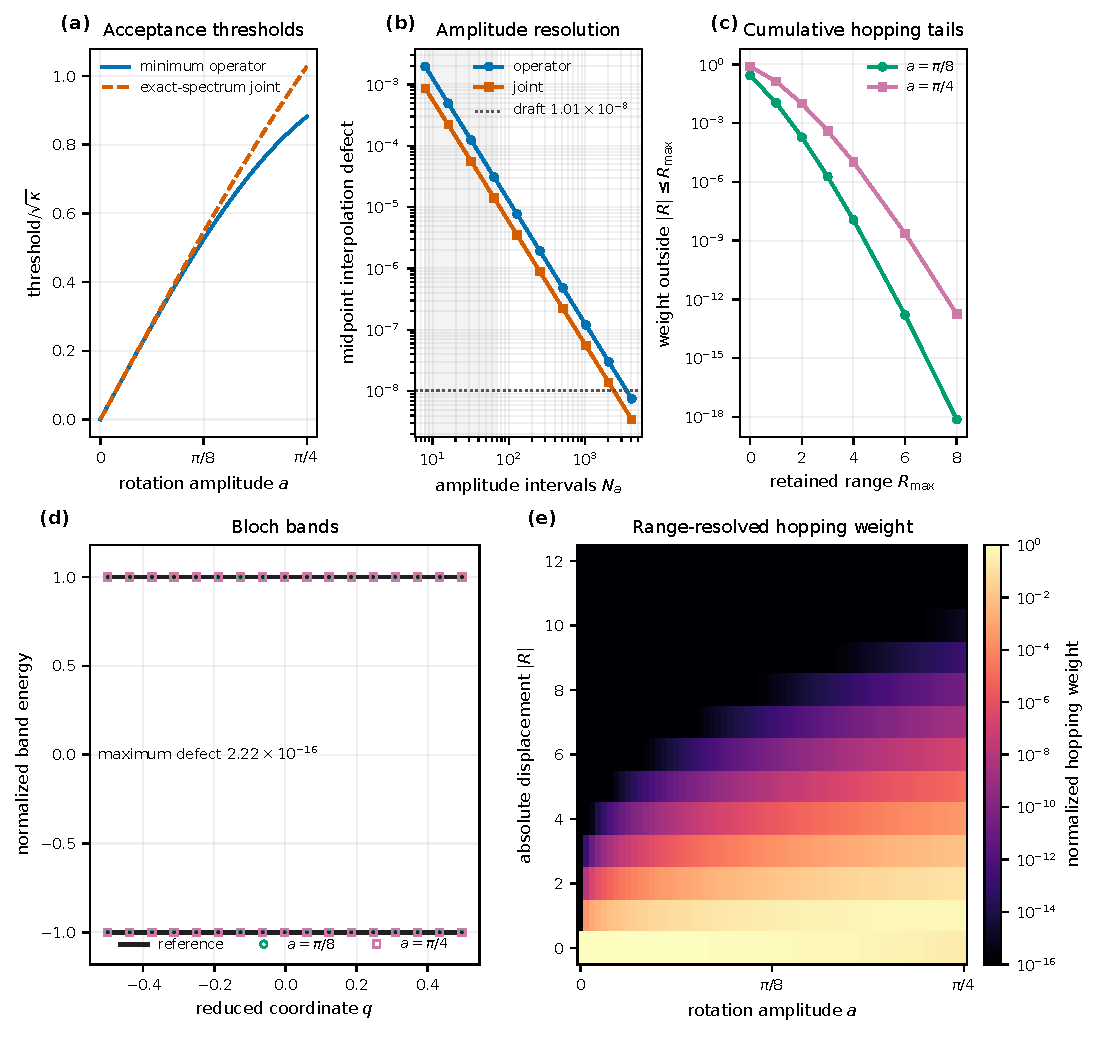
\includegraphics[width=\textwidth]
    {../../../../../experiments/model-adequacy/periodic1d/band-equivalence-versus-hopping-locality/analysis/band-equivalence-versus-hopping-locality.pdf}
  \caption{Band equivalence versus hopping locality in the smooth flat-parent
  continuum. \textbf{(a)} Normalized minimum operator and exact-spectrum joint
  acceptance thresholds as functions of the maximum rotation amplitude $a$.
  \textbf{(b)} Direct analytic correlation $\mu_{\max}(a)=J_0(2a)$; no amplitude
  interpolant is used for the continuum threshold claims.
  \textbf{(c)} Cumulative normalized hopping weight outside the retained range
  $|R|\le R_{\max}$ for two amplitudes. \textbf{(d)} Reference and transformed Bloch
  bands; the largest computed eigenvalue discrepancy is $2.22\times10^{-16}$.
  \textbf{(e)} Normalized range-resolved hopping weight over amplitude and absolute
  displacement. Thresholds in panel (a) use the analytic $J_0(2a)$ comparator; panels
  (c) and (e) use the $N=512$ finite transform after nested momentum refinement. The
  calculation is development analysis, not a retained evidence run.}
  \label{fig:flat-parent-analysis}
\end{figure}

\begin{figure}[p]
  \centering
  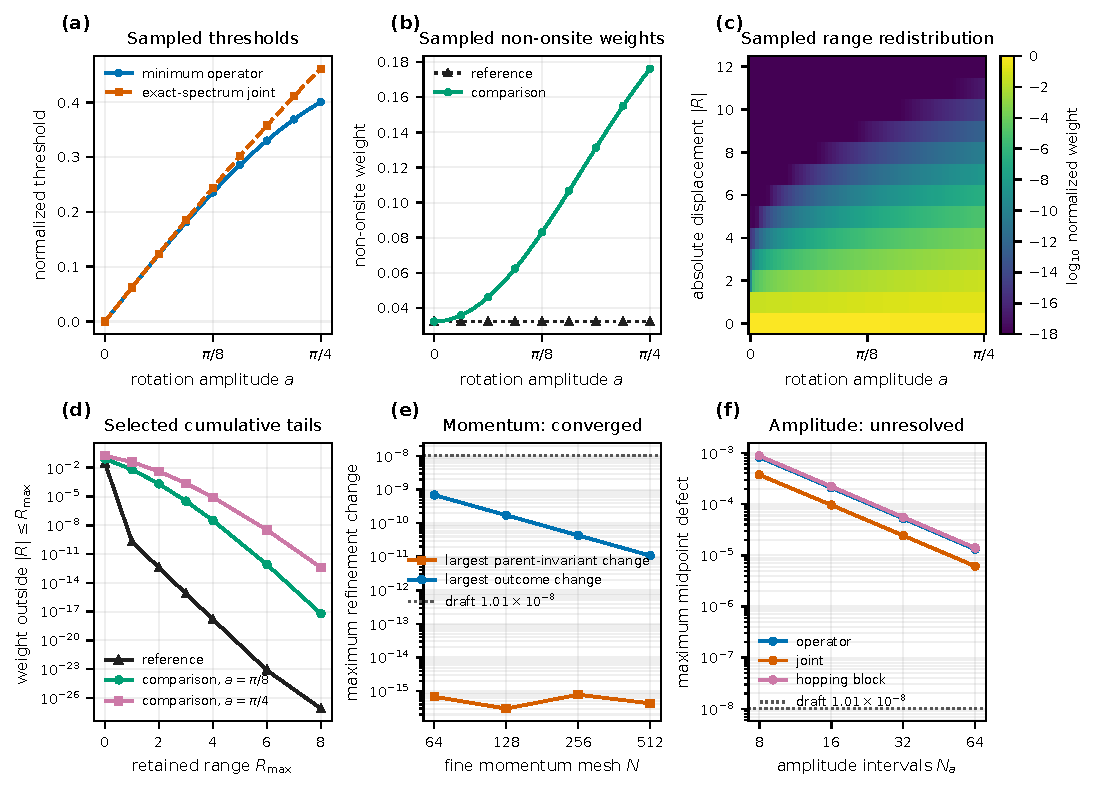
\includegraphics[width=\textwidth]
    {../../../../../experiments/model-adequacy/periodic1d/band-equivalence-versus-hopping-locality/analysis/nonflat-four-state-exploratory.pdf}
  \caption{Smooth non-flat four-state development calculation. \textbf{(a)}
  Restricted-alignment minimum-operator and exact-spectrum joint thresholds over a
  65-node sampling of the smooth amplitude family. Markers show every eighth direct
  sample and connecting lines are guides to the eye. \textbf{(b)} Reference and
  comparison non-onsite weights over the same samples.
  \textbf{(c)} Range-resolved comparison hopping redistribution over amplitude and
  absolute displacement. \textbf{(d)} Selected cumulative finite-mesh hopping tails.
  \textbf{(e)} Adjacent momentum-refinement changes: both parent-invariant and selected
  outcome channels lie below the draft target. \textbf{(f)}
  Midpoint amplitude-interpolation discrepancies, all above the draft target on the tested
  $N_a\le64$ ladder. No $J_0(2a)$ comparator or flat-parent residual--tail identity is
  used. Momentum refinement is `converged'; panel (f) motivates restricting the
  numerical conclusions to directly evaluated amplitudes rather than claiming a
  continuous interpolation. The calculation is not a retained evidence run.}
  \label{fig:nonflat-analysis}
\end{figure}

\begin{figure}[p]
  \centering
  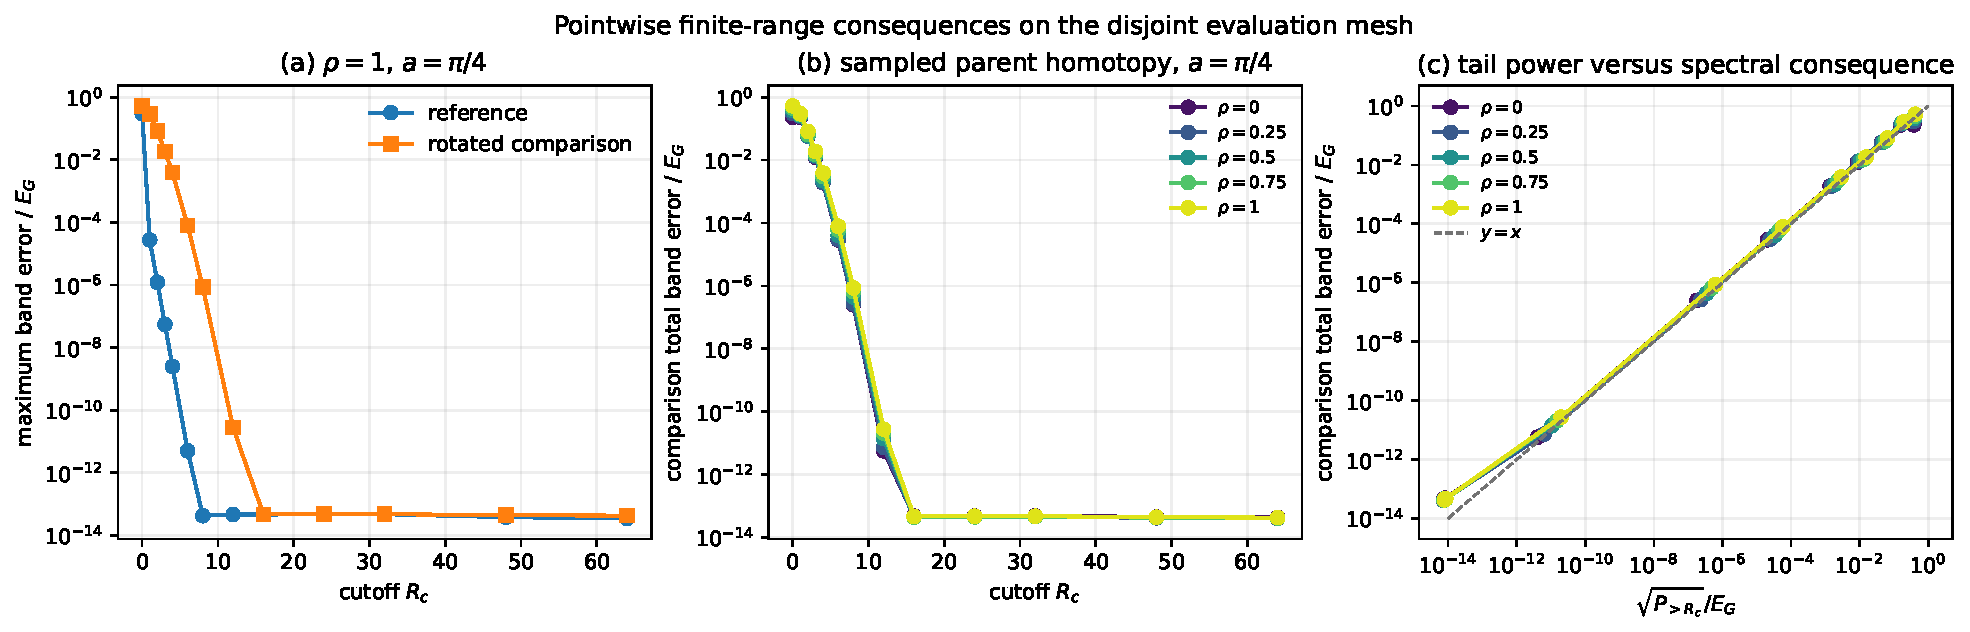
\includegraphics[width=\textwidth]
    {../../../../../experiments/model-adequacy/periodic1d/band-equivalence-versus-hopping-locality/analysis/truncation-band-consequences.pdf}
  \caption{Pointwise finite-range consequences after explicit ordinary-lattice
  truncation. \textbf{(a)} Maximum reference and rotated-comparison band errors for the
  dispersive endpoint $(\rho,a)=(1,\pi/4)$. \textbf{(b)} Comparison total band error
  across the five sampled parent scales at $a=\pi/4$. \textbf{(c)} Comparison total band
  error against the square root of total omitted block power; the dashed $y=x$ line is a
  visual comparator, not an identity or bound. The centered cyclic Nyquist block is
  removed and reported separately before PhysKit applies each conjugate-closed cutoff.
  Lines connect directly calculated cutoffs as guides to the eye. The binary64 floor,
  finite $\rho$ and amplitude samples, and lack of a frozen accuracy target preclude a
  continuous range-to-accuracy certificate. This is development analysis, not retained
  evidence or material validation.}
  \label{fig:truncation-consequences}
\end{figure}

\clearpage
\section{Retained scalar Fourier-reduction precursor}
\label{sec:retained-scalar-precursor}

A separate publication-independent experiment predates the active rank-two model-
adequacy calculation:
\begin{center}
\small
\path{ksdft2effmass.campaign.periodic-reduction.periodic1d.single-band-fourier-reduction.v1}\par
\path{ksdft2effmass.campaign.periodic-reduction.periodic1d.single-band-fourier-reduction.v1.run-20261014T184707Z}.
\end{center}
It is a retained local synthetic run with strict schemas, content-addressed evidence,
independent direct-formula verification, and exact historical-channel parity. The
cutoff-five plane-wave discrepancy is
$5.3113069498067489\times10^{-13}E_G$. The finite-difference discrepancies on 31- and
255-point grids are $1.7532741974955801\times10^{-2}E_G$ and
$2.5977169467195083\times10^{-4}E_G$, respectively. Complete transform reconstruction
closes to $4.1661377054983873\times10^{-17}E_G$, and the range-eight maximum error on
the disjoint evaluation mesh is $9.4652957589869136\times10^{-9}E_G$. The maximum
independent energy and squared-energy reconstruction defects are
$2.7311486405778851\times10^{-14}E_G$ and
$9.2157184661267877\times10^{-19}E_G^2$.

\begin{figure}[htbp]
  \centering
  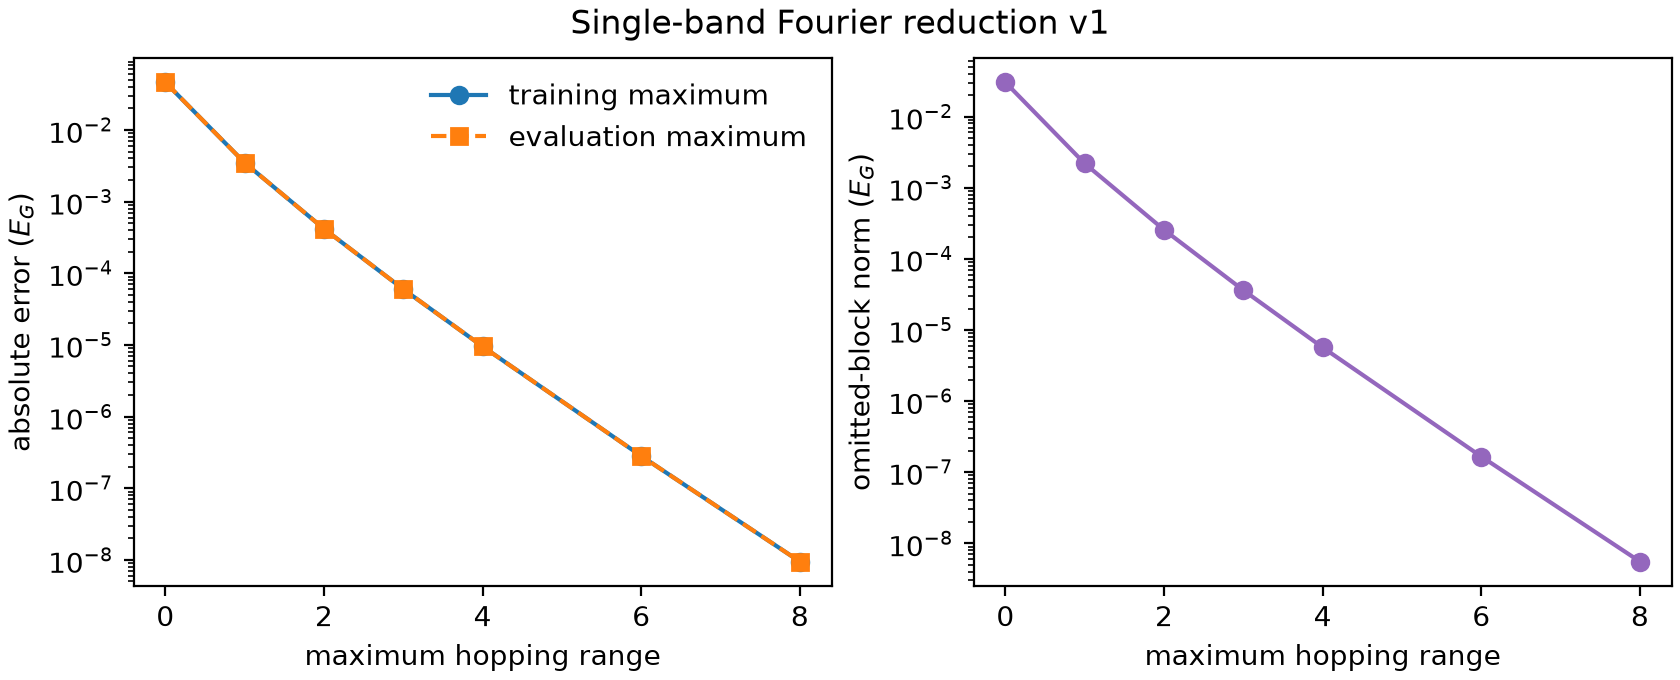
\includegraphics[width=0.96\textwidth]
    {../../../../../experiments/periodic-reduction/single-band-fourier-reduction/periodic1d/runs/ksdft2effmass.campaign.periodic-reduction.periodic1d.single-band-fourier-reduction.v1.run-20261014T184707Z/single-band-fourier-reduction-summary.png}
  \caption{Retained one-dimensional single-band Fourier-reduction control. The panels
  report finite-difference, plane-wave, Fourier-reconstruction, and finite-range
  channels under the experiment's own versioned contract. This retained scalar evidence
  is not an execution of the active rank-two model-adequacy protocol.}
  \label{fig:retained-single-band-precursor}
\end{figure}

The sampled exterior gaps, finite-grid errors, and range inventory remain finite-protocol
quantities. They are not continuum isolation certificates, a scientifically selected
hopping range, material validation, or evidence for the rank-two range-inflation result.
The scalar run is included to expose the verified reduction-chain precursor rather than
to pool its error channels with the active experiment.

\clearpage
\section{Exact rectangle minimization}

For
\[
 f(p)=(p-p_c)^TQ(p-p_c)+m,
 \qquad
 Q=
 \begin{pmatrix}Q_{11}&Q_{12}\\Q_{12}&Q_{22}\end{pmatrix},
\]
the unconstrained center is included when it lies in $X$. On a vertical edge $p_1=b$,
the unconstrained edge minimizer is
\[
 p_2=p_{c,2}-\frac{Q_{12}}{Q_{22}}(b-p_{c,1}),
\]
which is clipped to $[\lambda_{\min},\lambda_{\max}]$. This is done for
$b=s_{\min}$ and $b=s_{\max}$. On a horizontal edge $p_2=b$, the corresponding minimizer
is
\[
 p_1=p_{c,1}-\frac{Q_{12}}{Q_{11}}(b-p_{c,2}),
\]
clipped to $[s_{\min},s_{\max}]$. Direct evaluation of the original quadratic at these
points yields the exact rectangle minimum for a positive-definite two-dimensional
quadratic. Corners appear automatically when clipping reaches an endpoint.

\section{Support and containment checks}

For a general quadratic ellipse
\[
 \mathcal E=\{p:(p-p_c)^TQ(p-p_c)\le\beta\},
 \qquad Q\succ0,
\]
the support point and support value in direction $d\ne0$ are
\begin{align}
 p_+(d)&=p_c+
 \sqrt{\frac{\beta}{d^TQ^{-1}d}}Q^{-1}d,\\
 \max_{p\in\mathcal E}d^Tp
 &=d^Tp_c+\sqrt{\beta\,d^TQ^{-1}d}.
\end{align}
Coordinate extrema are obtained using $d=(1,0)^T$ and $d=(0,1)^T$ together with their
negatives. Containment requires all four extrema to remain within the corresponding box
bounds after accounting for the fixed containment tolerance. The support calculation
uses linear solves with $Q$ and never substitutes a box-clipped point into a formula for
the full ellipse. For the common curvature in
Theorem~\ref{main-thm:exact-loss-geometry}, these checks reduce to the semiaxes stated by
Eqs.~\eqref{main-eq:exact-spectral-loss} and \eqref{main-eq:exact-operator-loss}.

A candidate upper bound on the distance is computed from an explicitly feasible pair
$(p_s,p_o)$ as $\norm{p_s-p_o}_2$. A projected lower bound is accepted only after its
support points, component orientation, containment premise, and threshold membership
have been independently reconstructed. The inequalities
\[
 0\le\underline\delta\le\delta^*\le\overline\delta
\]
must hold within numerical tolerance. A violation indicates a calculation or premise
failure, not an unusual scientific result.

\section{Execution sequence}

The confirmatory calculation follows the sequence below without adaptive changes to the
scientific controls.

\begin{enumerate}
  \item Parse canonical input and reject unknown, malformed, nonfinite, or inconsistent
        fields.
  \item Construct $K(q)$ on every mesh in the declared refinement ladder.
  \item Diagonalize the parent, retain the lowest two states, and verify the external
        gap and retained projectors.
  \item Build and periodically close the transported frame; stop on deficient overlap.
  \item Construct $H(q)$ and the complete amplitude family $A_a(q)$ and retain all
        parent diagnostics.
  \item For every momentum and amplitude mesh, construct the spectral quadratic and the
        exact second-harmonic operator correlation from the original residuals.
  \item Maximize the continuous harmonic over its half-open fundamental interval,
        record unique or degenerate angle status, construct the optimized operator
        quadratic, and minimize both quadratics over the fixed parameter rectangle.
  \item Apply all continuous and discrete convergence gates. Stop with failed
        qualification if the declared caps are reached first.
  \item Freeze the selected construction resolution without changing thresholds or
        parameter bounds.
  \item Search for a common witness and verify it from the original residuals.
  \item If no witness is established, test every separation-certificate premise and
        construct conservative lower and upper bounds.
  \item Assign the disposition from construction data and the declared numerical
        uncertainty rules.
  \item Generate the disjoint evaluation mesh and compute evaluation losses without
        changing the disposition.
  \item Transform the reference, comparison, and selected candidate matrices to hopping
        blocks and calculate range-resolved locality norms.
  \item Serialize canonical evidence, perform independent reconstruction, validate
        schemas and digests, and retain the package only if all required checks pass.
\end{enumerate}

\bibliographystyle{unsrt}
\bibliography{references}

\end{document}
